\documentclass[aspectratio=169]{beamer}

\newif\ifmore
\morefalse

\usepackage{inputenc}[utf8]
\usepackage[polish]{babel}

%Lepiej tego nie zmieniaj, jak co to dodawaj pakiety
\usepackage{fancyhdr}
\usepackage{mdframed}
\usepackage{graphicx}
\usepackage{listings}
\usepackage{caption}
\usepackage{float}
\usepackage{tikz}
\usepackage{xcolor}
\usetikzlibrary{arrows}
\usepackage{hyperref}
\hypersetup{
    colorlinks=false,
    linkcolor=blue,
    filecolor=magenta,      
    urlcolor=cyan,
}
%\apptocmd{\frame}{}{\justifying}{} % Allow optional arguments after frame.

\urlstyle{same}
%Zmienne, zmień je!
\graphicspath{ {./ilustracje/} }
\title[BFC64]{Brainfuck Compiler 64 - Programowanie bardzo niskopoziomowe.}
\author{Grzegorz Koperwas}
\date{\today}

%lokalizacja polska (odkomentuj jak piszesz po polsku)

\usepackage{polski}
\usepackage[polish]{babel} 
\usepackage{indentfirst}
\usepackage{icomma} 
\usetheme{Warsaw}

\brokenpenalty=1000
\clubpenalty=1000
\widowpenalty=1000    

%nie odkometowuj wszystkiego, użyj mózgu
%\renewcommand\thechapter{\arabic{chapter}.}
\renewcommand\thesection{\arabic{section}.}
\renewcommand\thesubsection{\arabic{section}.\arabic{subsection}.}
\renewcommand\thesubsubsection{\arabic{subsubsection}.}

%Makra

\newcommand{\obrazek}[2]{
\begin{figure}[h]
    \centering
    \includegraphics[scale=#1]{#2}
\end{figure}
}     
        

\newcommand{\twierdzonko}[1]{
    \begin{center}
    \begin{mdframed}
    #1
    \end{mdframed}          
    \end{center}
} 

\newcommand{\dwanajeden}[2]{
\ensuremath \left( \begin{array}{c}
    #1\\
    #2
\end{array} \right)
}  

\lstdefinestyle{asm}{
    frame=trBL,
    numbers=left,
    basicstyle=\ttfamily\footnotesize,
    keywordstyle=\color{orange},
    morekeywords={lda,sta,jsr,ldy,clc,adc,jmp,stx,cmp,beq,iny,sty}
}

\lstdefinestyle{tinyasm}{
    frame=trBL,
    numbers=left,
    basicstyle=\ttfamily\scriptsize,
    keywordstyle=\color{orange},
    morekeywords={lda,sta,jsr,ldy,clc,adc,jmp,stx,cmp,beq,iny,sty}
}
\captionsetup[figure]{name=Załącznik}

\begin{document}
\begin{frame}
    \titlepage
\end{frame}
\begin{frame}
    \tableofcontents
\end{frame}
\section{Jak napisać kompilator?}
\begin{frame}
    \frametitle{Jak napisać kompilator?}
    Zanim zaczniemy pisać kompilator musimy sobie odpowiedzieć na parę pytań:

    \begin{description}
        \item[Czemu?] \pause By móc mówić że napisałem kompilator.
        \item[Czego?] \pause Brainfuck'a - języka stworzonego by twórca mógł mówić że napisał kompilator w 256 bajtach.
        \item[Na co?] \pause Commodore 64 - Ten 40 letni assembler nie może być taki trudny.
    \end{description}
\end{frame}
\subsection{Czym jest Brainfuck?}
\begin{frame}[fragile]
    \frametitle{Brainfuck 101}
    \begin{columns}
        \begin{column}{0.5\textwidth}
            \textbf{Brainfuck} - jak sama nazwa wskazuje nie jest zbytnio czytelnym językiem.

            Brainfuck nie posiada koncepcji zmiennej, zamiast tego oferuje nam \emph{dużą} taśmę z komórkami na zmienne liczbowe.


        \end{column}
        \begin{column}{.5\textwidth}
            Jego cała składnia składa się nie z słów, jak w \texttt{c++}, tylko z paru znaków:

            \begin{description}
                \item[{$<$}, {$>$}] Przesuń taśmę w lewo/prawo
                \item[+, -] Dodaj/Odejmnij 1 od komórki pamięci
                \item[., ,] Wypisz/wczytaj znak do komórki pamięci
                \item[{[, ]}] Pętla \texttt{while~(komórka~!=~0)}.
            \end{description}
        \end{column}
    \end{columns}
\end{frame}
\begin{frame}[fragile]
    \frametitle{Przykładowy program:}
    \begin{lstlisting}[frame=L,basicstyle=\footnotesize\ttfamily,numbers=left]
++++++++
[
    >++++
    [
        >++>+++>+++>+<<<<-
    ]
    >+>+>->>+
    [<]
    <-
]
>>.>---.+++++++..+++.>>.<-.<.+++.------.--------.>>+.>++.
            \end{lstlisting}
    \pause
    Jak ktoś pomyślał że to ,,Hello World'' to gratulacje.
\end{frame}

\subsection{Jak działa BFC64}
\begin{frame}[fragile]
    \frametitle{Jak działa BFC64?}
    \begin{columns}
        \begin{column}{0.8\textwidth}
            \textbf{BFC64} składa się z trzech części:
            \begin{description}
                \item[Parsera] Zamienia on znaki bf na \texttt{Symbol}e \pause
                \item[Optymalizatora] Procesor może dodawać liczby, można to wykorzystać.\pause 
                \item[Kompilator] Generuje kod assemblera w oparciu o wzorce \pause
            \end{description}
            \pause
            Funkcje assemblera oraz linkera spełnia \texttt{kickassembler}.
        \end{column}
        \begin{column}{0.2\textwidth}
            \begin{tikzpicture}[scale=.7]
                \draw (0,2) rectangle (4, 3);
                \node at (2,2.5){Plik .bf};
                \draw [->, thick] (2,2) -- (2,1);

                \draw (0,0) rectangle (4,1);
                \node at (2,.5){BFC64};
                \draw [->, thick] (2,0) -- (2,-1);

                \draw (0,-2) rectangle (4, -1);
                \node at (2,-1.5){Plik .asm};
                \draw [->, thick] (2,-2) -- (2,-3);

                \draw (0,-4) rectangle (4, -3);
                \node at (2,-3.5){KickAssembler};
                \draw [->, thick] (2,-4) -- (2,-5);

                \draw (0,-6) rectangle (4, -5);
                \node at (2,-5.5){Plik .prg};
            \end{tikzpicture}
        \end{column}
    \end{columns}
\end{frame}
\begin{frame}
    \frametitle{Czym są te wzorce}
    \textbf{Kompilator} w BFC64 działa poprzez wklejanie za kolejne \texttt{symbol}e fragmentów assemblera.

    Wykorzystuje on również stos w celu przydzielania odpowiednich referencji końcom pętli (koniec pętli musi wiedzieć gdzie się ona zaczyna)
    \pause
    \vspace{5mm}

    Same fragmenty assemblera wkleja w odpowiednie miejsca skrypt \emph{pythona} podczas kompilacji. Czyta on pliki z odpowiedniego folderu i zamienia on je na funkcje \texttt{c++} za pomocą wzorca.
\end{frame}
\begin{frame}[fragile]
    \frametitle{Czemu skrypt pythona?}
    \begin{lstlisting}[language=c++,style=asm,showstringspaces=false,stringstyle=\color{red},identifierstyle=\color{blue},firstnumber=69]
std::string
subtract(std::string value, std::string label, std::string label2)
    {
        return "    lda ($fb),y\n    clc\n    cmp #" + value
               + "\n    bcs " + label + " //if lower than "
               + "number\n    lda #$00\n    jmp " + label2
               + "\n" + label + ":\n    sec\n    sbc #" + value
               + "\n" + label2 + ":\n    sta ($fb),y\n";
    }
        \end{lstlisting}
\end{frame}
\section{Programowanie \emph{bardzo niskopoziomowe}}
\subsection{Architektura Commodore64}
\begin{frame}
    \frametitle{Podstawy architektury \texttt{MOS 6510} w \texttt{Commodore 64}}
    \begin{columns}
        \begin{column}{0.5\textwidth}
            Co musimy znać by móc programować w assemblerze: \pause
            \begin{itemize}
                \item Zestaw instrukcji procesora \pause
                \item Urządzenia wejścia wyjścia \pause
                \item Mapę pamięci komputera \pause
                \item Kernal lub bios lub system operacyjny (cokolwiek jest dostępne) \pause
            \end{itemize}
        \end{column}
        \begin{column}{0.5\textwidth}
            \textbf{Commodore 64} nie posiada żadnego systemu operacyjnego, posiada za to \texttt{BASIC}'a oraz Kernal w pamięci \texttt{ROM}.

            \pause \vspace{5mm}

            \textbf{Kernal} jest takim odpowiednikiem \emph{biblioteki systemowej}, zawiera funkcje do łatwiejszego wypisywania znaków na ekran i wczytywania ich z klawiatury.
        \end{column}
    \end{columns}
\end{frame}

\ifmore
    \begin{frame}
        \frametitle{Mapy pamięci}
        \textbf{Procesory} mogą czytać i zapisywać bezpośrednio nie tylko do pamięci \texttt{RAM}

        \pause\vspace{5mm}

        Jako iż komodorek nie posiada systemu operacyjnego, to mamy dowolność w wyborze gdzie co damy, poza paroma wymogami: \pause
        \begin{itemize}
            \item Program zaczyna się na adresie \texttt{\$4000}. \pause
            \item Pointery działają tylko w pierwszych 256 bajtach.\pause
            \item Kolejne 256 bajtów to stos procesora.\pause
            \item Część pamięci to pamięć ROM z kernalem, można ją zamienić na \texttt{RAM}, ale my go potrzebujemy.\pause
            \item Część pamięci przechowuje takie informacje jak tekst na ekranie, kolor tekstu, inna część to porty szeregowe, klawiatura itp.
        \end{itemize}
    \end{frame}
\fi

\begin{frame}
    \frametitle{Procesor \texttt{MOS 6510/6502}}
    Procesor w Commodore 64 posiada cztery ośmiobitowe rejestry:\pause
    \begin{description}
        \item[X oraz Y] - rejestry którymi możemy indeksować pamięć
        \item[A] - Akumulator, na nim są przeprowadzane operacje matematyczne
        \item[S] - wskaźnik do stosu (rozmiar to 256 bajtów/128 adresów)
    \end{description}
    \pause
    Procesor może dodawać oraz odejmować. Może Dokonywać operacji bitowych (and, or, shift, rotate) oraz porównywać liczby, wynik zapisuje jako flagi.

    \pause\vspace{5mm}

    Procesor jest 8 bitowy, ale posiada 16 bitową szynę danych (max 64 kilobajty pamięci). Przez to wskaźniki mogą być tylko w pamięci \emph{zeropage} (pierwsze 256 bajtów).
\end{frame}

\subsection{Hello world w asemblerze}

\begin{frame}
    \frametitle{Assembler 6502 101}
    Assembler używa mnemonik, skrótów nazw instrukcji procesora, na przykład:\pause
    \begin{description}
        \item[\texttt{LDA}] LoaD A
        \item[\texttt{JSR}] Jump SubRoutine
        \item[\texttt{INY}] INcrease Y
    \end{description}
    \pause
    Assembler nie posiada pętli, mamy do dyspozycji tylko skoki (goto) lub skoki warunkowe.

    \pause\vspace{5mm}

    Różne mnemoniki posiadają różne sposoby adresowanie argumentów, mogą być to sztywne adresy, adresy względne, indeksowanie rejestrami czy indeksowanie wskaźników rejestrami.
\end{frame}
\begin{frame}[fragile]
    \lstinputlisting[style=asm]{helloworld.asm}
\end{frame}

\subsection{Jak wyglądają wzorce}
\begin{frame}
    \frametitle{Jak wyglądają wzroce w porównaniu do \texttt{c++}}
    \begin{columns}
        \begin{column}{0.6\textwidth}
            Mamy taki wzorzec:
            \lstinputlisting[style=tinyasm,numbers=none]{inc.asm}
            \footnotesize{
                Gdzie:
                \begin{itemize}
                    \item \texttt{\$FB} - pointer do pointera taśmy
                    \item Rejestr \texttt{Y} to indeks taśmy
                    \item Za \texttt{label()} kompilator wsadza jakąś nazwę
                \end{itemize}
                \pause
            }
        \end{column}
        \begin{column}{0.4\textwidth}
            W \texttt{c++}:
            \lstinputlisting[language=c,style=tinyasm,numbers=none]{inc.cpp}
            \footnotesize{
                Gdzie:
                \begin{itemize}
                    \item \texttt{tapeptr} - \texttt{int*} - wskaźnik do taśmy
                    \item \texttt{i} - \texttt{int} - indeks taśmy
                \end{itemize}
            }
        \end{column}
    \end{columns}
\end{frame}

\section{Podsumowanie}
\subsection{Inne wzorce}
\begin{frame}
    \frametitle{Inne wzorce}
    Dla każdego symbolu robimy kolejne wzorce:
    \begin{description}
        \item[$<$, $>$] - Zmniejsz/zwiększ rejestr \texttt{Y}, jeśli jest równy od 0/255, zmniejsz/zwiększ bardziej znaczący bajt pointera.
        \item[.] - Załaduj wartość do \texttt{A}, skocz do funkcji wypisującej z Kernala.
        \item[,] - Skacz do funkcji wczytującej z Kernala aż \texttt{A != 0}
        \item[{[}] - Załaduj wartość do \texttt{A}, jeśli \texttt{A == 0} to skocz do końca pętli
        \item [{]}] - Skocz do początku pętli
    \end{description}
\end{frame}

\subsection{Koniec}
\begin{frame}
    Po tym wszystkim pozostaje jedno pytanie:
    \pause\vspace{2cm}
    \begin{center}
        \Large{\textbf{\color{blue}W czym napisano assemblera?}}
    \end{center}
    \vspace{3cm}
    \begin{flushright}
        \tiny{\textit{Papier++ go brrrrr}}
    \end{flushright}
\end{frame}
\subsection{Materiały}
\begin{frame}
    \frametitle{Materiały}
    \begin{columns}
        \begin{column}{.6\textwidth}
            \begin{itemize}
                \item \href{https://eater.net/}{Filmiki Ben'a Eater'a o budowaniu komputera i karty graficznej na płytkach prototypowych}
                \item \href{https://www.masswerk.at/6502/6502_instruction_set.html}{Zestaw instrukcji 6502}
                \item Dokumentacja KickAssemblera
                \item \href{https://github.com/HakierGrzonzo/bfc64}{Dokumentacja oraz kod na Github'ie}
            \end{itemize}
        \end{column}
        \begin{column}{.4\textwidth}
            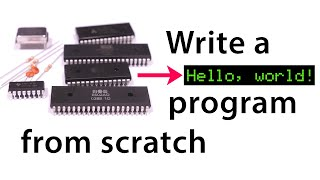
\includegraphics[scale=.5]{6502YT.jpg}
        \end{column}
    \end{columns}
\end{frame}
\end{document}
